\documentclass[9pt]{article}
\usepackage[letterpaper,margin=0.48in]{geometry}
\usepackage{booktabs,tabularx,array,xcolor,tikz,multicol,hyperref}
\usetikzlibrary{arrows.meta,positioning}
\pagestyle{empty}
\setlength{\parindent}{0pt}
\setlength{\parskip}{2.5pt}
\setlength{\columnsep}{0.22in}
\renewcommand{\arraystretch}{1.08}
\definecolor{hnavy}{HTML}{112B45}
\definecolor{hblue}{HTML}{1E78B4}
\definecolor{hgreen}{HTML}{167C63}
\definecolor{hpale}{HTML}{EAF4F8}
\definecolor{hred}{HTML}{A4423D}
\hypersetup{colorlinks=true,urlcolor=hblue}

\begin{document}
\begin{tabularx}{\textwidth}{@{}Xr@{}}
{\Large\bfseries\color{hnavy} Horizon Mechanistic Interpretability: H1--H5} &
{\small\bfseries Development evidence --- 24 September 2026}
\end{tabularx}

\vspace{2pt}\colorbox{hpale}{\parbox{0.985\textwidth}{\small
\textbf{Boundary.} These monitors measure WaSR-T perception health. They do not
prove free water, create metric obstacles, steer the vessel, or authorize
actuation. Missing context or calibration returns \texttt{unknown}.}}

\vspace{4pt}
\begin{tabularx}{\textwidth}{@{}>{\bfseries}p{0.42in}p{2.55in}X p{1.43in}@{}}
\toprule
ID & Experiment & Development result & Meaning now \\
\midrule
H1 & Exposure, blur, freeze, timing, horizon, occlusion, and output-change checks.
& No complete frames in the first 296-frame run because independent horizon and occlusion evidence was absent.
& Transparent deterministic checks; deliberately incomplete. \\
H2 & Diagonal Mahalanobis distance on a grouped 64-dimensional encoder summary.
& Median 7.233; 95th percentile 11.995.
& Descriptive novelty; no calibrated fault threshold. \\
H3 & PCA reconstruction of the same grouped representation.
& Median error 0.01233; 95th percentile 0.02409.
& Nonlinear-shift baseline, not mechanistic evidence. \\
H4 & SAE on all 2,048 pooled final-encoder channels, followed by matched interventions.
& Validated 64-feature direction beat both controls in 15/18 trials ($p=0.00377$). A better-reconstructing 96-feature model failed at 11/18 ($p=0.240$).
& One bounded causal direction; no temporal mechanism or semantic label. \\
H5 & Hard-TopK temporal-fusion SAE with temporal training, cross-seed feature stability, and matched causal controls.
& Selected feature beat both controls in 18/18 trials ($p=3.81\times10^{-6}$); minimum decoder cosine 0.528 and activation correlation 0.667.
& Strongest development signal; product-integrated but shadow-only. \\
\bottomrule
\end{tabularx}

\vspace{5pt}
\begin{multicols}{2}
{\large\bfseries\color{hnavy} How H5 works}

\begin{center}
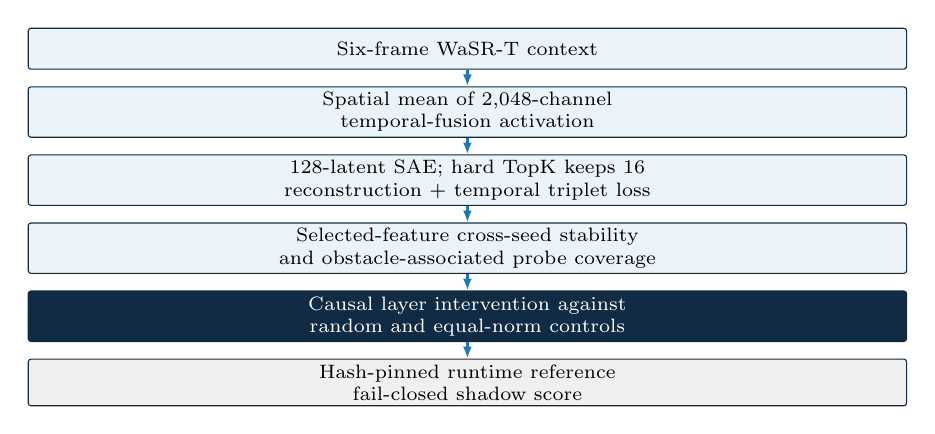
\begin{tikzpicture}[node distance=2.1mm,every node/.style={font=\scriptsize,align=center},box/.style={draw=hnavy,rounded corners=1pt,minimum width=.92\columnwidth,minimum height=5.2mm,inner sep=2pt},arr/.style={-{Latex[length=1.5mm]},hblue,thick}]
\node[box,fill=hpale] (a) {Six-frame WaSR-T context};
\node[box,fill=hpale,below=of a] (b) {Spatial mean of 2,048-channel\\temporal-fusion activation};
\node[box,fill=hpale,below=of b] (c) {128-latent SAE; hard TopK keeps 16\\reconstruction $+$ temporal triplet loss};
\node[box,fill=hpale,below=of c] (d) {Selected-feature cross-seed stability\\and obstacle-associated probe coverage};
\node[box,fill=hnavy,text=white,below=of d] (e) {Causal layer intervention against\\random and equal-norm controls};
\node[box,fill=gray!12,below=of e] (f) {Hash-pinned runtime reference\\fail-closed shadow score};
\draw[arr] (a)--(b); \draw[arr] (b)--(c); \draw[arr] (c)--(d);
\draw[arr] (d)--(e); \draw[arr] (e)--(f);
\end{tikzpicture}
\end{center}

H5 observes the model after temporal fusion rather than at its image encoder.
Adjacent frames are positive pairs; the corresponding sampled position from
another sequence is the negative. Exact TopK sparsity limits each state to at
most 16 active latents. The selected direction must match independently trained
replicas before its intervention outcomes are considered.

\columnbreak
{\large\bfseries\color{hnavy} What the experiment found}

The selected 128-latent model converged in 622 epochs with 3 dead features.
Against an identical zero-temporal-weight baseline:

\begin{tabular}{@{}lr@{}}
Validation reconstruction MSE & $0.9533\rightarrow0.8295$ \\
Cross/adjacent distance ratio & $6.12\rightarrow6.89$ \\
Whole-dictionary mean cosine & 0.425 (poor) \\
Selected-feature minimum cosine & 0.528 (pass) \\
Selected-feature minimum correlation & 0.667 (pass) \\
Causal-control wins & 18/18 (pass) \\
\end{tabular}

Two earlier development runs revealed weak whole-dictionary stability and
informed the feature-specific gate. The successful rerun is therefore
development evidence, not a sealed confirmatory result.

{\large\bfseries\color{hnavy} Product status}

H5 is wired into the shared health contract, product launcher, monitor registry,
and recorded-camera pipeline. The launcher verifies a SHA-256-pinned external
reference and refuses altered, missing, or method-mismatched artifacts. The
first frame is unknown until temporal context exists; later scores remain
unknown without a frozen calibration artifact. H5 cannot increase A5 authority.

\textbf{Still required before authority:} fault-labelled calibration and a
false-alarm target; sealed H1--H5 held-out comparison; target-computer latency
and resource qualification; spatial localization and collateral-effect tests.

{\footnotesize\textbf{Research basis.} Temporal coherence:
\href{https://arxiv.org/abs/2604.03919}{Dokme and Vishwanath (2026)};
visual SAE localization: \href{https://arxiv.org/abs/2412.05276}{Lim et al.};
causal feature circuits: \href{https://arxiv.org/abs/2403.19647}{Marks et al.};
activation patching: \href{https://arxiv.org/abs/2404.15255}{Heimersheim and Nanda}.
All numerical results use the frozen \texttt{kope81} development collection.}
\end{multicols}
\end{document}
